\section{Experiments}

\subsection{Setup}

We consider five different NLP datasets. They are ``ag news'', ``dbpedia'', ``yahoo answers'', ``amazon review'', ``amazon review''(see appendix~\ref{} for details of the datasets).  Our continual learning setup comprises of two type of tasks, 1-Individual task-shuffled label, 2-Sequential datasets.

\paragraph{Individual task-shuffled label:}
% In this type of the continual learning, we consider each individual dataset separately. This is corresponding to shuffled label in vision tasks~\cite{}. For each of them, we define a sequence of tasks as a sequence of new label assignment. Basically, for the given dataset, we permute the labels for the first task, then the model will learn it. Then for the second task we use the same dataset and permute its label and so on. 
In this continual learning paradigm, we treat each dataset independently. This approach is analogous to the shuffled label method used in vision tasks~\cite{}. For each dataset, we define a sequence of tasks through a series of label permutations. Specifically, for a given dataset, we permute the labels for the first task, which the model then learns. For subsequent tasks, we use the same dataset with different permutations of the labels and this continues until end of the learning.


\paragraph{Sequential datasets:}
% In this type of the continual learning, we consider a sequence of the datasets as a sequence of the tasks. In this way, we will have dataset one, dataset two,  ..., dataset five, dataset one, dataset two, ... and so on. 
In this continual learning paradigm, we treat a sequence of datasets as a sequence of tasks. This involves using dataset one, followed by dataset two, and so on up to dataset five, before repeating the sequence from dataset one. This repeats forever.

using the common head for type two.

put figure to explain them

\paragraph{Type of the Networks:}
To investigate the behavior of plasticity, we conduct experiments using different types of networks. These include ``Bert-transformer'', ``MLP'', ``Conv'', ``LSTM'', ``Multi-head Attention layer'',  ``Multi-head Attention layer with residual connection'', and ``one Bert-layer without dropout''.
Except for the \textit{BERT-Transformer}, all other networks consist of three layers: the first layer is an embedding layer, and the last layer is a classifier layer. The middle layer corresponds to the specific type of network being tested. We keep the number of hidden units the same across them and equal to $50$.We chose this setting to simplify the neural networks and investigate plasticity in NLP tasks .


To conduct a comprehensive evaluation of optimizers and learning rates, we considered three optimizers: Adam, AdamW, and SGD. For each optimizer, we varied the learning rate between $10^{-2}$ and $10^{-5}$.

For the \textit{BERT-Transformer}, we used the base size and two optimizers Adam and AdamW. We also consider {\color{red}XX} as the learning rates.

% \begin{itemize}
% \item What is the datasets,
% \item  models,
% \item CL setup: number of tasks,
% \item optimizers, hyper-param setup (details about the grid search over lr).
% \item Random label ( 100\%, 50\%, 20\%)
% \end{itemize}
% Also, mention why did you choose this particular setup.


\subsection{Results with Transformer (default setup)}

The first experiment we conducted focused on the ability of continual learning, plasticity, in the BERT transformer. In this experiment, we used both pretrained and non-pretrained BERT models to assess the impact of pretraining on plasticity.

\subsubsection{Effect of pre-training - pre trained bert}
\autoref{fig:nlp_bert_pretrained}
\begin{itemize}
    \item Bert Model (pre-trained and no-pretrained)
    \item is that because of pretrained and non-pretrained
    \item is that because of transformers?
          datasets % \item is that because of scale?
\end{itemize}
% --- is that because of pretrained and non-pretrained 

% --- is that because of transformers

\begin{figure*}[htb!]
    \centering
    \resizebox{\textwidth}{!}{
        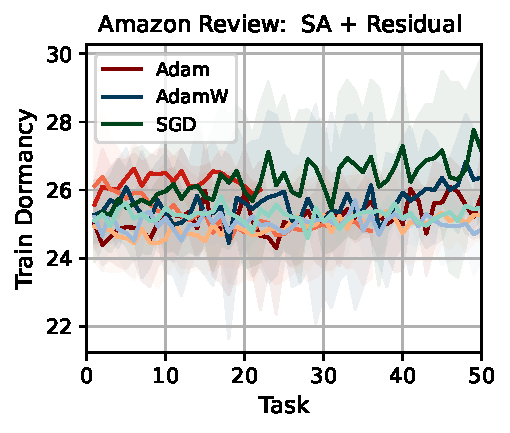
\includegraphics[width=\textwidth]{figs/Accuracy/nlp/transformer_pretrained/amazon_review_full_40.pdf}
        \includegraphics[width=\textwidth]{figs/Accuracy/nlp/transformer_pretrained/yahoo_answers_40.pdf}
        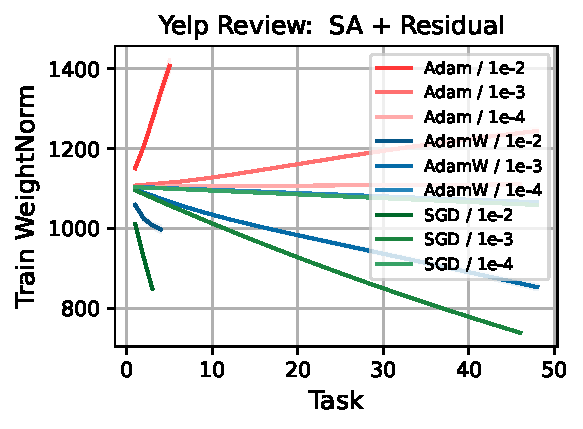
\includegraphics[width=\textwidth]{figs/Accuracy/nlp/transformer_pretrained/yelp_review_full_40.pdf}
        % \includegraphics[width=\textwidth]{figs/Accuracy/nlp/transformer_pretrained/dbpedia_40.pdf}
    }
    % \\
    % \resizebox{\textwidth}{!}{  
    % 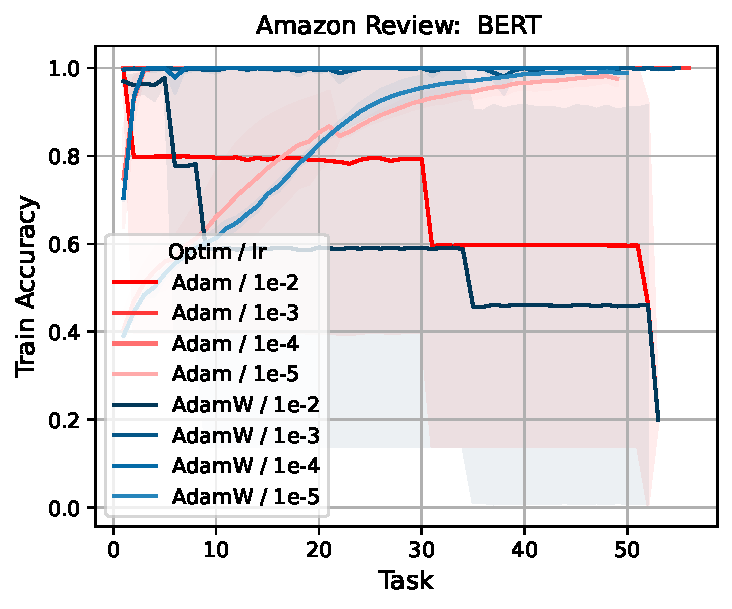
\includegraphics[width=\textwidth]{figs/Accuracy/nlp/bert/amazon_review_full_40.pdf}
    % 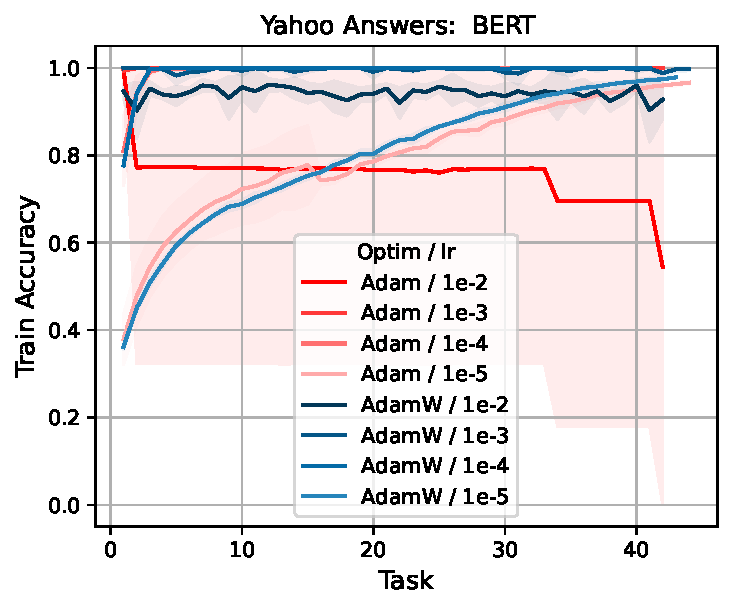
\includegraphics[width=\textwidth]{figs/Accuracy/nlp/bert/yahoo_answers_40.pdf}
    % 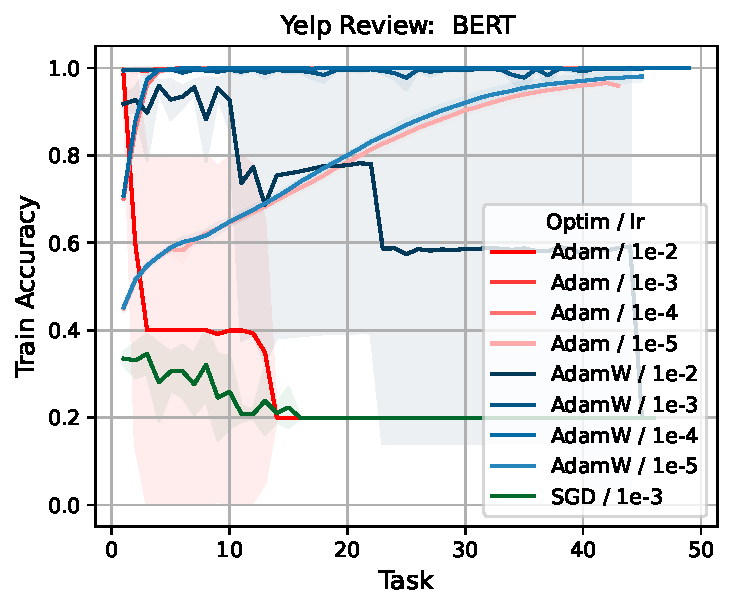
\includegraphics[width=\textwidth]{figs/Accuracy/nlp/bert/yelp_review_full_40.pdf}
    % % 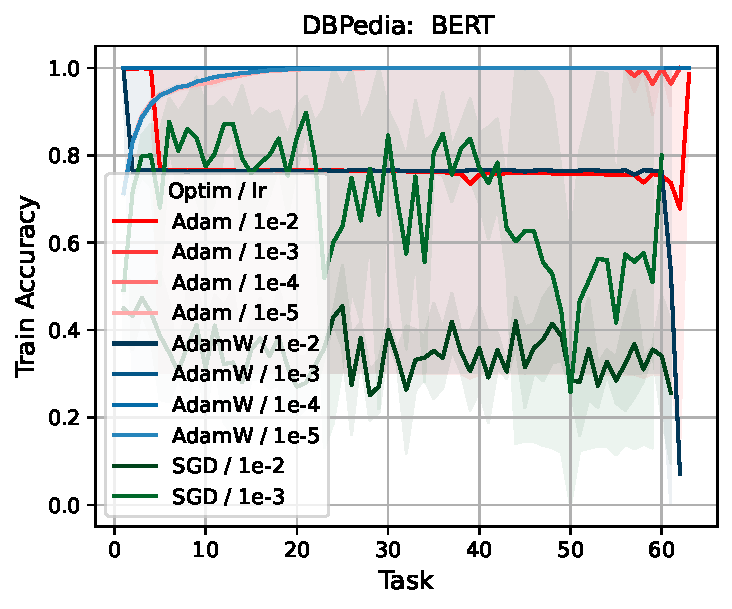
\includegraphics[width=\textwidth]{figs/Accuracy/nlp/bert/dbpedia_40.pdf}
    % }
    \caption{Accuracy of BERT pretrained on NLP datasets.}
    \label{fig:nlp_bert_pretrained}
\end{figure*}


% \subsection{Ablations/Intervention/Analysis}

\subsection{Experiments for other type of networks: CNN, LSTM}

To further explore plasticity in NLP datasets, we conducted experiments using various types of networks, including MLP, CNN, and LSTM.

\autoref{fig:nlp_mlp} shows the results of the MLP network for the NLP datasets for both \textit{Individual task-shuffled label} and \textit{Sequential datasets} compared to CIFAR-10. As tasks continue, there is no loss of plasticity for the NLP datasets, whereas there is loss of plasticity for CIFAR-10.


For the CNN experiments with NLP datasets, the network maintains plasticity when using the Adam and AdamW optimizers, but it loses the plasticity with SGD, \autoref{fig:nlp_cnn}. This contrasts with the results for image datasets~\cite{plasticity papers}, as we also demonstrated for CIFAR-10. For image datasets, the network is unable to learn new tasks after a while, even when using Adam and AdamW.

\autoref{fig:nlp_lstnm} shows the learning curves for the LSTM network. Both \textit{Individual tasks-shuffled label} and \textit{Sequential datasets} maintain plasticity. Surprisingly, in this case, with CIFAR-10 LSTM also has plasticity and the performance does not decrease.


% Surprisingly, as shown in \autoref{fig:nlp_lstnm}, in LSTM network, 

% add ---> \autoref{fig:nlp_mlp} 5 for each data and one for cifar

\autoref{fig:nlp_cnn_lstm}
\begin{itemize}
    \item CNN on NLP results. Is there plasticity loss?
    \item LSTM on NLP results. Is there plasticity loss?
\end{itemize}



--> mention that we only look at training in this scenario not test or validation and this is different from catastrophic forgetting

\begin{figure*}[htb!]
    \centering
    \resizebox{\textwidth}{!}{
        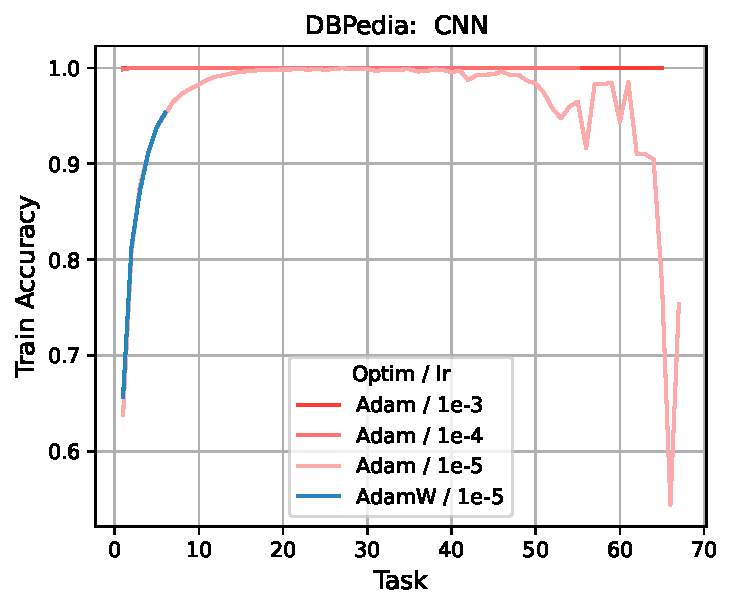
\includegraphics[width=\textwidth]{figs/Accuracy/nlp/cnn/dbpedia_50.pdf}
        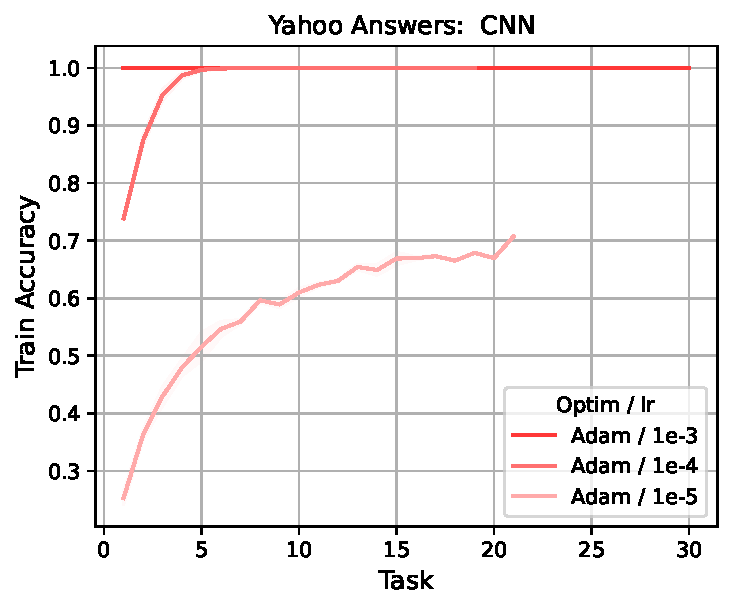
\includegraphics[width=\textwidth]{figs/Accuracy/nlp/cnn/yahoo_answers_50.pdf}
        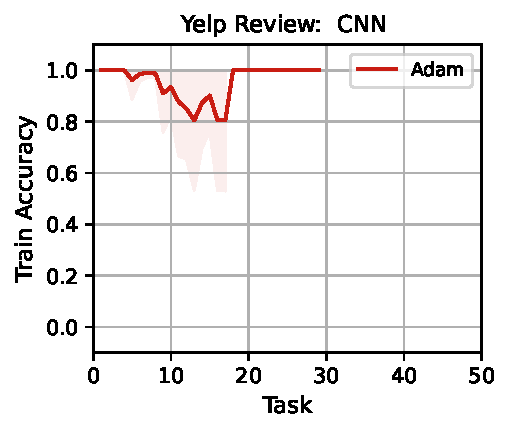
\includegraphics[width=\textwidth]{figs/Accuracy/nlp/cnn/yelp_review_full_50.pdf}
    }
    \\
    \resizebox{\textwidth}{!}{
        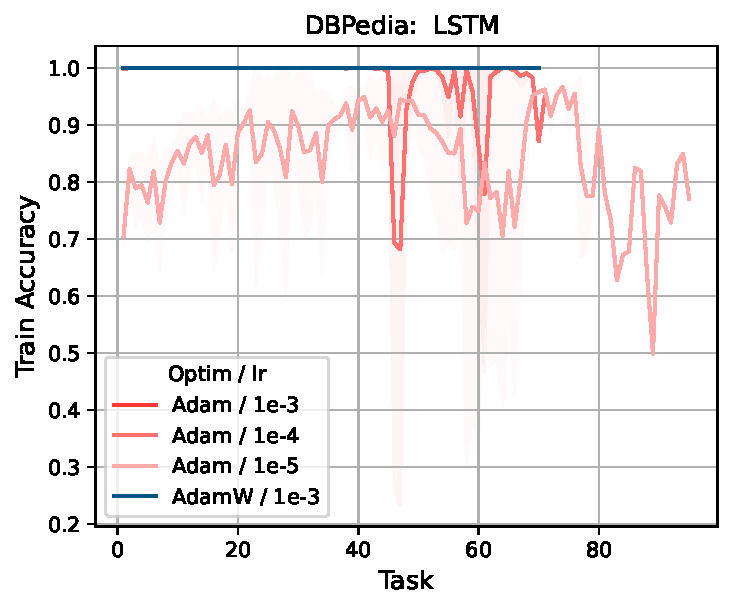
\includegraphics[width=\textwidth]{figs/Accuracy/nlp/lstm/dbpedia_50.pdf}
        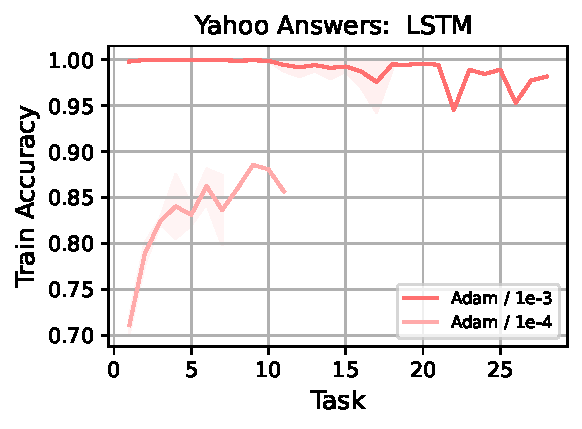
\includegraphics[width=\textwidth]{figs/Accuracy/nlp/lstm/yahoo_answers_50.pdf}
        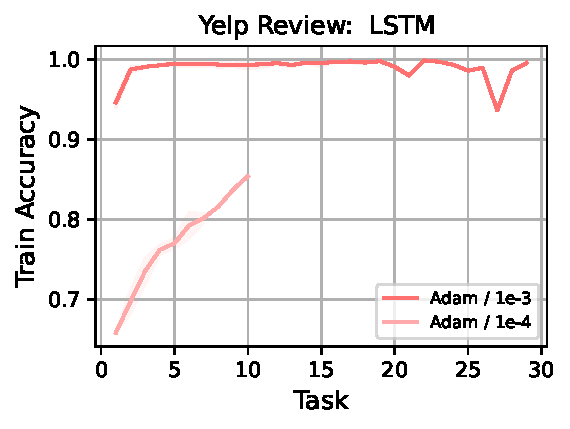
\includegraphics[width=\textwidth]{figs/Accuracy/nlp/lstm/yelp_review_full_50.pdf}
    }
    \caption{Accuracy of CNN and LSTM on NLP datasets.}
    \label{fig:nlp_cnn_lstm}
\end{figure*}

Analysis: \autoref{fig:yahoo_models_analysis}
\begin{figure*}[htb!]
    \centering
    \resizebox{\textwidth}{!}{
        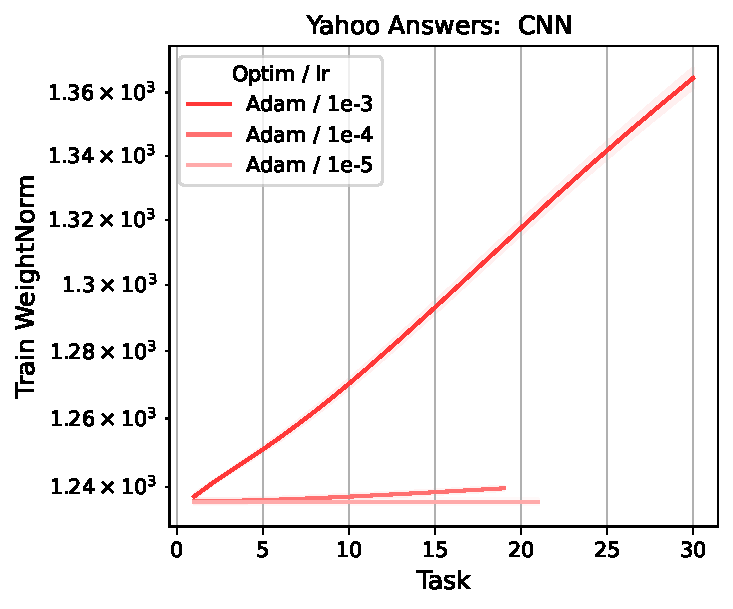
\includegraphics[width=\textwidth]{figs/WeightNorm/nlp/cnn/yahoo_answers_50.pdf}
        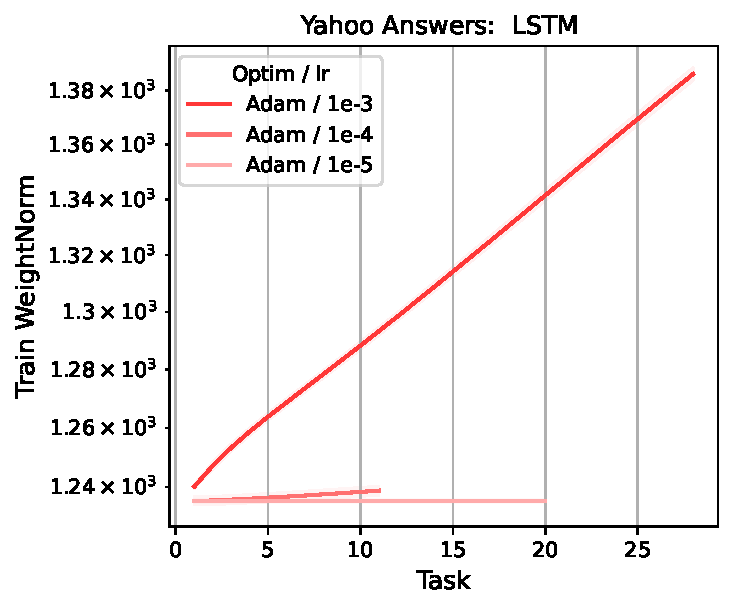
\includegraphics[width=\textwidth]{figs/WeightNorm/nlp/lstm/yahoo_answers_50.pdf}
        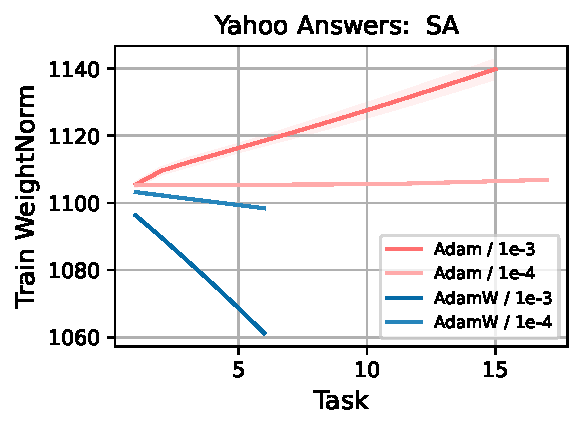
\includegraphics[width=\textwidth]{figs/WeightNorm/nlp/attention/yahoo_answers_40.pdf}
        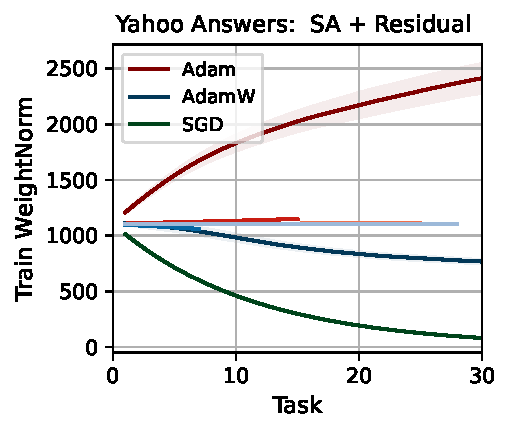
\includegraphics[width=\textwidth]{figs/WeightNorm/nlp/attention_residual/yahoo_answers_40.pdf}
        \includegraphics[width=\textwidth]{figs/WeightNorm/nlp/bert_layer/yahoo_answers_40.pdf}
    }\\    \resizebox{\textwidth}{!}{
        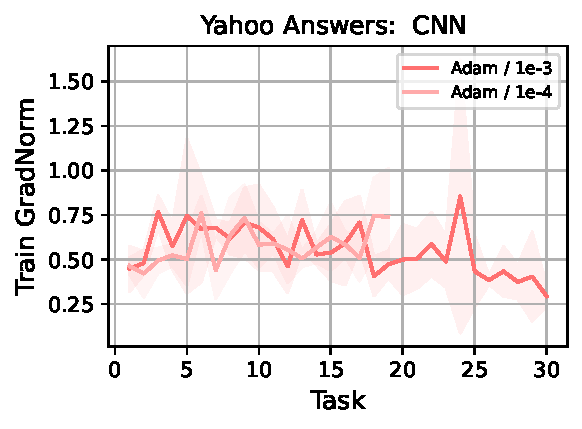
\includegraphics[width=\textwidth]{figs/GradNorm/nlp/cnn/yahoo_answers_50.pdf}
        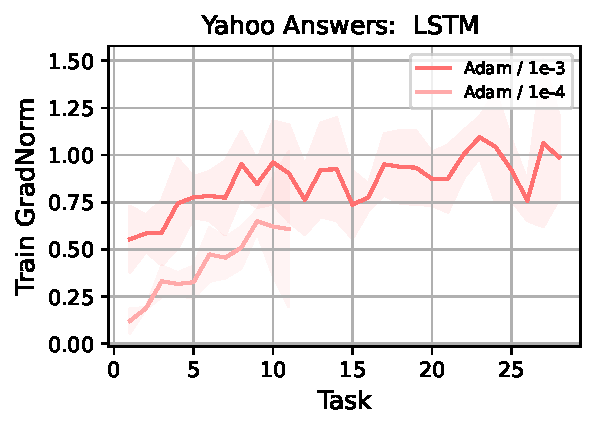
\includegraphics[width=\textwidth]{figs/GradNorm/nlp/lstm/yahoo_answers_50.pdf}
        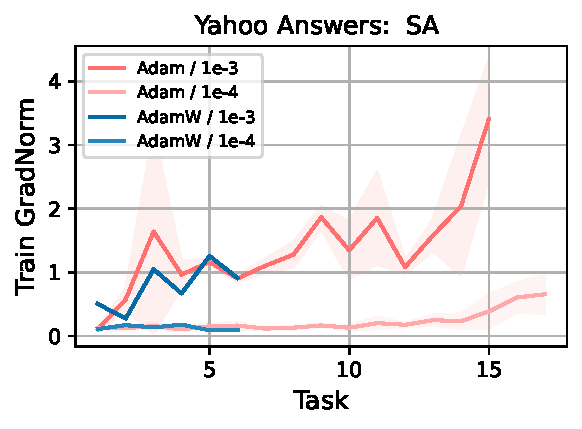
\includegraphics[width=\textwidth]{figs/GradNorm/nlp/attention/yahoo_answers_40.pdf}
        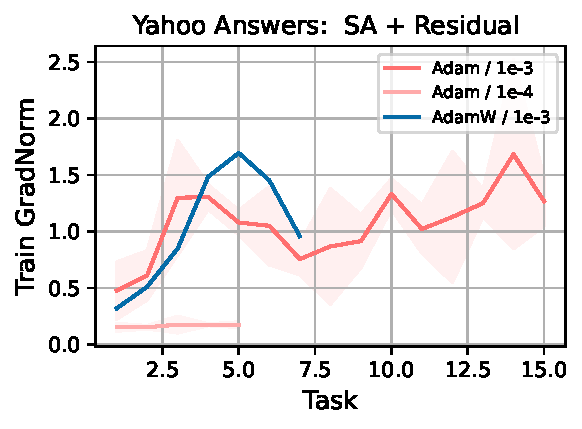
\includegraphics[width=\textwidth]{figs/GradNorm/nlp/attention_residual/yahoo_answers_40.pdf}
        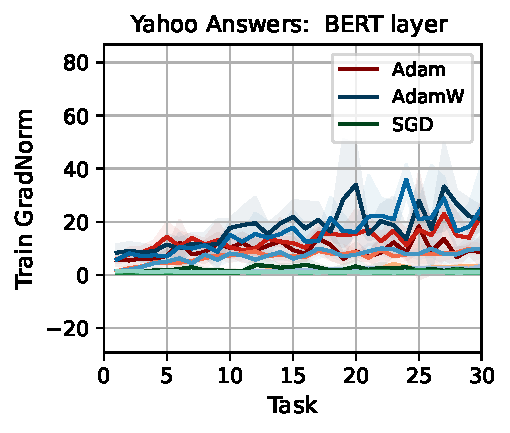
\includegraphics[width=\textwidth]{figs/GradNorm/nlp/bert_layer/yahoo_answers_40.pdf}
    }\\
    \resizebox{\textwidth}{!}{
        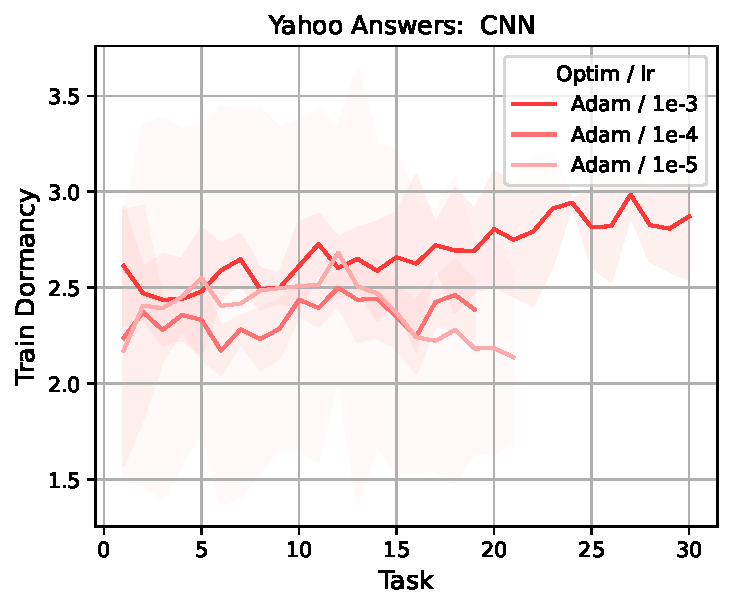
\includegraphics[width=\textwidth]{figs/Dormancy/nlp/cnn/yahoo_answers_50.pdf}
        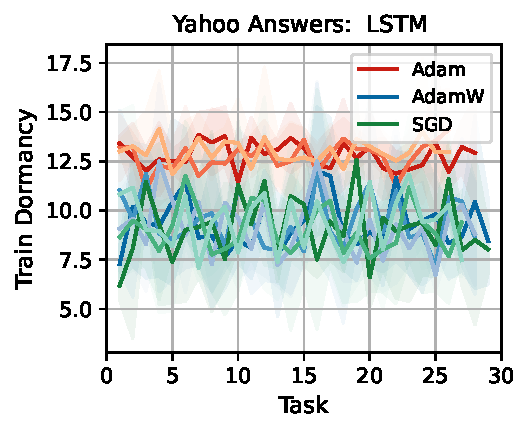
\includegraphics[width=\textwidth]{figs/Dormancy/nlp/lstm/yahoo_answers_50.pdf}
        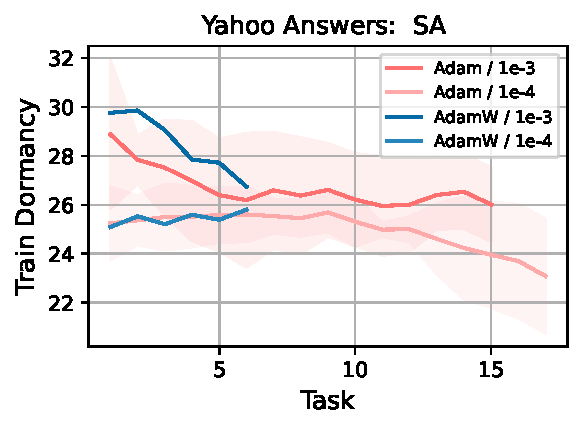
\includegraphics[width=\textwidth]{figs/Dormancy/nlp/attention/yahoo_answers_40.pdf}
        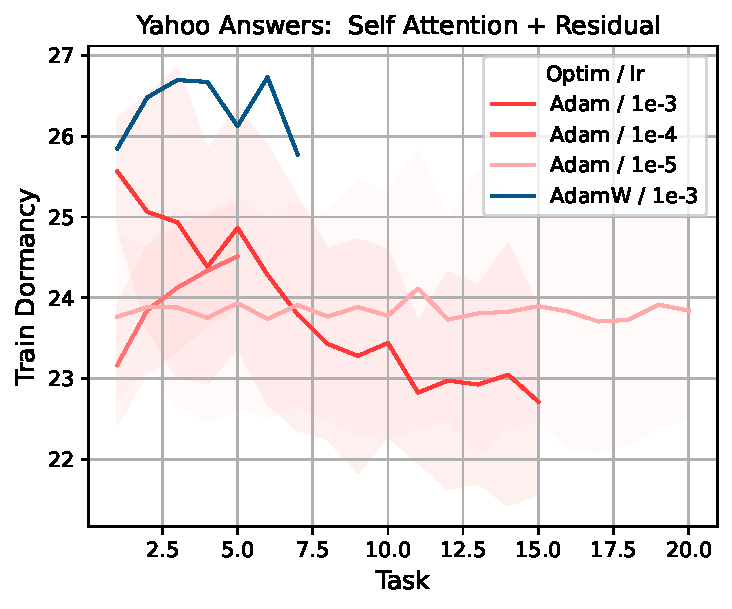
\includegraphics[width=\textwidth]{figs/Dormancy/nlp/attention_residual/yahoo_answers_40.pdf}
        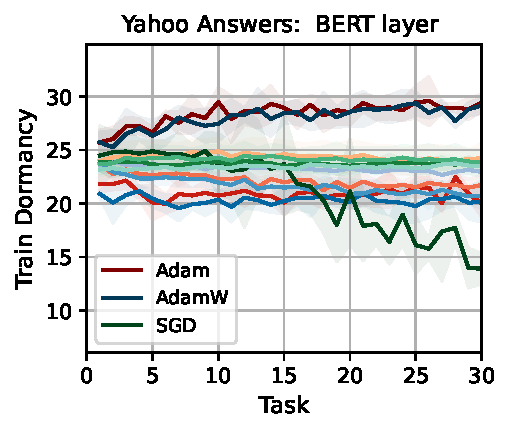
\includegraphics[width=\textwidth]{figs/Dormancy/nlp/bert_layer/yahoo_answers_40.pdf}
    }
    \caption{Analysis of different models on Yahoo Answers datasets.}
    \label{fig:yahoo_models_analysis}
\end{figure*}



\subsection{Comparison with vision}

\autoref{fig:image_models}
\begin{figure*}[t]
    \centering
    \resizebox{\textwidth}{!}{
        % 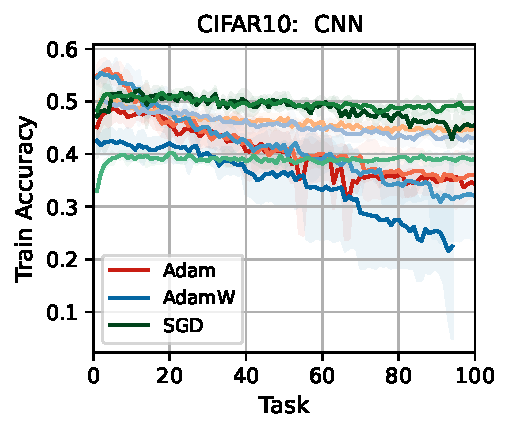
\includegraphics[width=\textwidth]{figs/Accuracy/image/cnn/cifar10_50.pdf}
        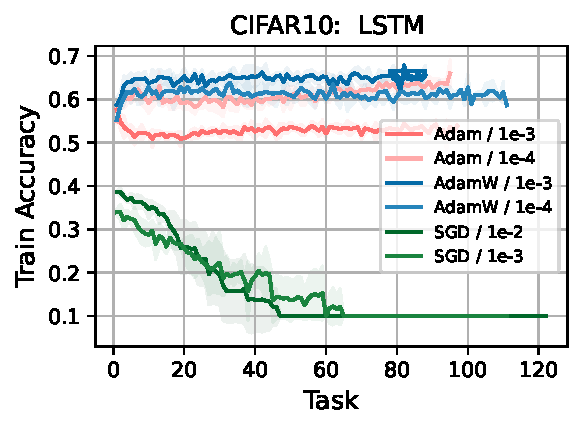
\includegraphics[width=\textwidth]{figs/Accuracy/image/lstm/cifar10_50.pdf}
        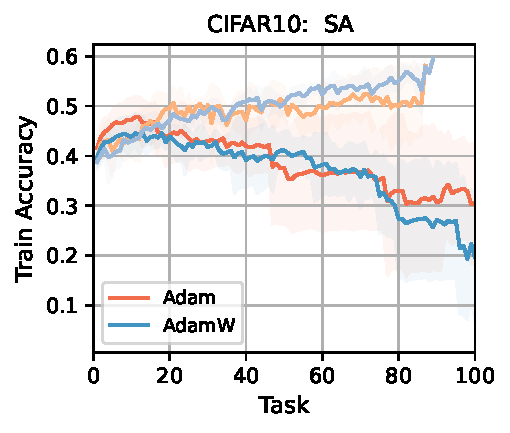
\includegraphics[width=\textwidth]{figs/Accuracy/image/attention/cifar10_40.pdf}
        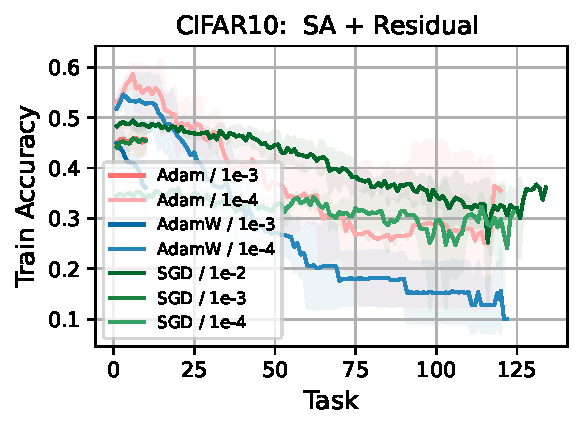
\includegraphics[width=\textwidth]{figs/Accuracy/image/attention_residual/cifar10_40.pdf}
    }
    \caption{Accuracy of different models on CIFAR10.}
    \label{fig:image_models}
\end{figure*}



\subsubsection{self-attention vs MLP}

\autoref{fig:nlp_self_res}
\begin{itemize}
    \item Self Attention Layer (Embedding + Multi-head Attention layer + Classifier)
    \item Self Attention Layer  with Residual Layer
    \item Bert Layer( Layer Norm and dropout)
\end{itemize}


\begin{figure*}[t]
    \centering
    \resizebox{\textwidth}{!}{
        % 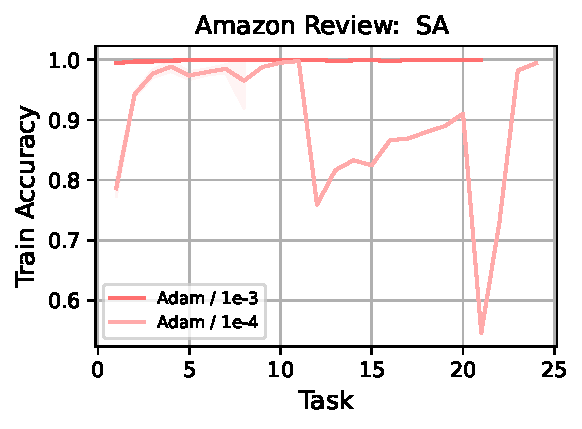
\includegraphics[width=\textwidth]{figs/Accuracy/nlp/attention/amazon_review_full_40.pdf}
        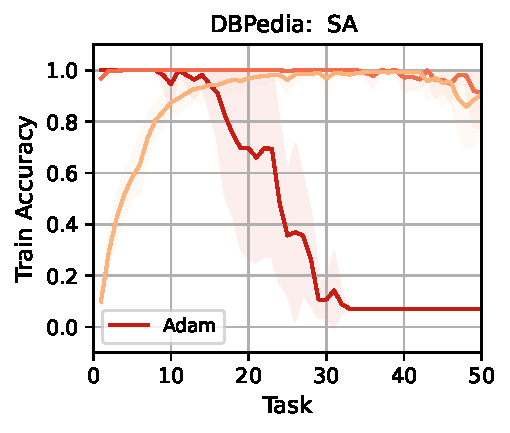
\includegraphics[width=\textwidth]{figs/Accuracy/nlp/attention/dbpedia_40.pdf}
        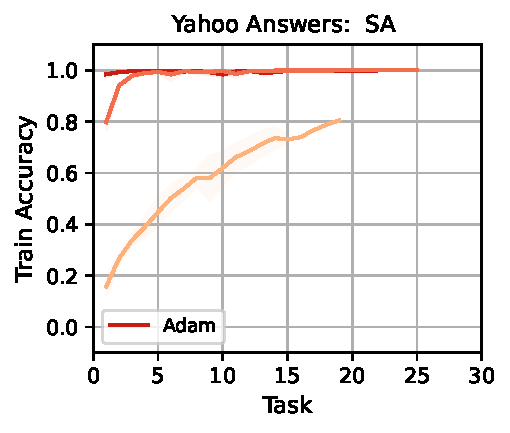
\includegraphics[width=\textwidth]{figs/Accuracy/nlp/attention/yahoo_answers_40.pdf}
        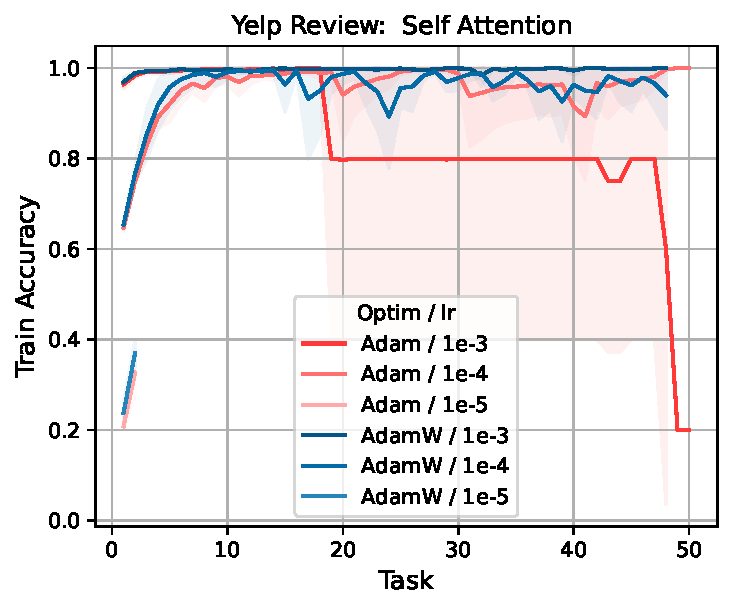
\includegraphics[width=\textwidth]{figs/Accuracy/nlp/attention/yelp_review_full_40.pdf}
    }
    \\
    \resizebox{\textwidth}{!}{
        % 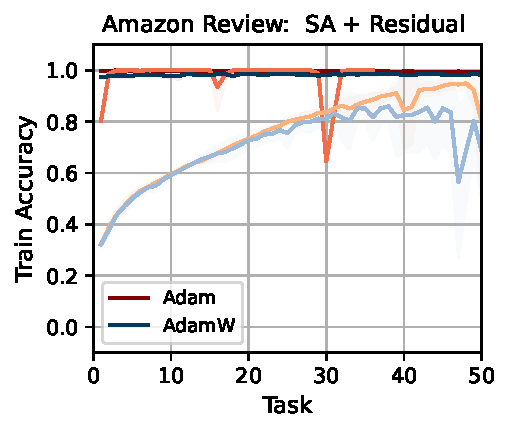
\includegraphics[width=\textwidth]{figs/Accuracy/nlp/attention_residual/amazon_review_full_40.pdf}
        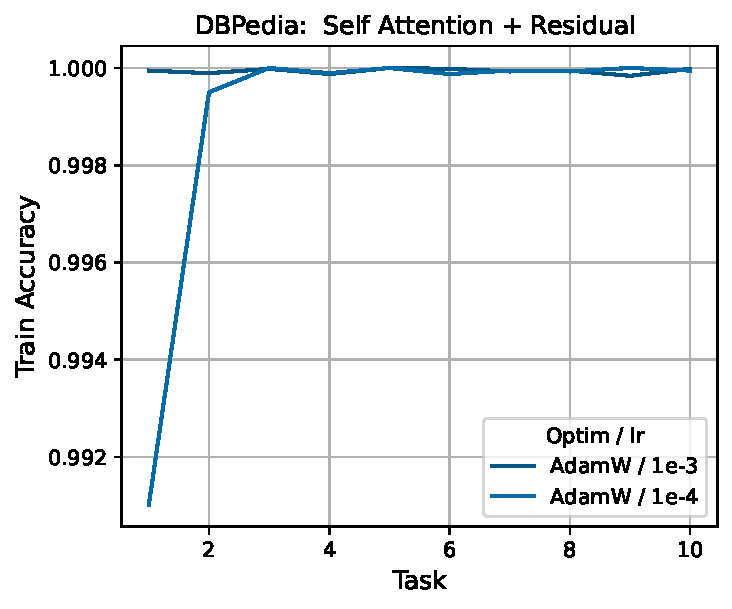
\includegraphics[width=\textwidth]{figs/Accuracy/nlp/attention_residual/dbpedia_40.pdf}
        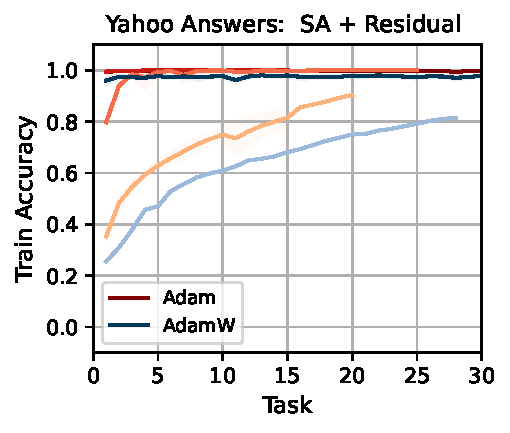
\includegraphics[width=\textwidth]{figs/Accuracy/nlp/attention_residual/yahoo_answers_40.pdf}
        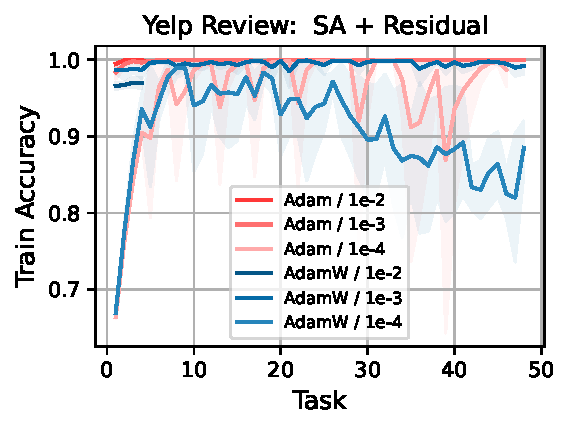
\includegraphics[width=\textwidth]{figs/Accuracy/nlp/attention_residual/yelp_review_full_40.pdf}
    }
    \\
    \resizebox{\textwidth}{!}{
        % 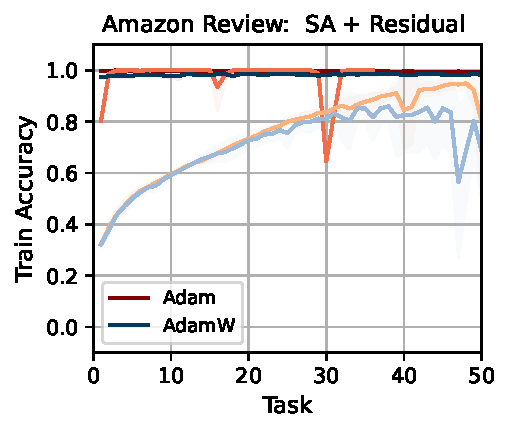
\includegraphics[width=\textwidth]{figs/Accuracy/nlp/attention_residual/amazon_review_full_40.pdf}
        \includegraphics[width=\textwidth]{figs/Accuracy/nlp/bert_layer/dbpedia_40.pdf}
        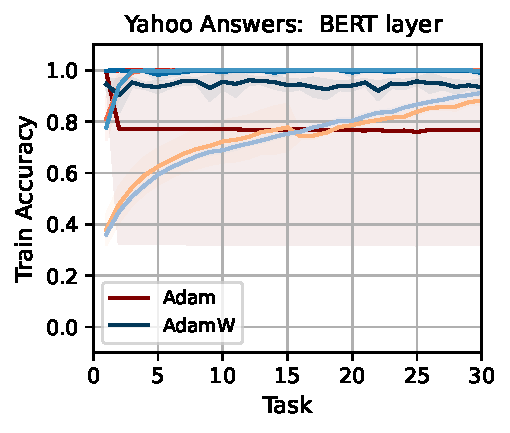
\includegraphics[width=\textwidth]{figs/Accuracy/nlp/bert_layer/yahoo_answers_40.pdf}
        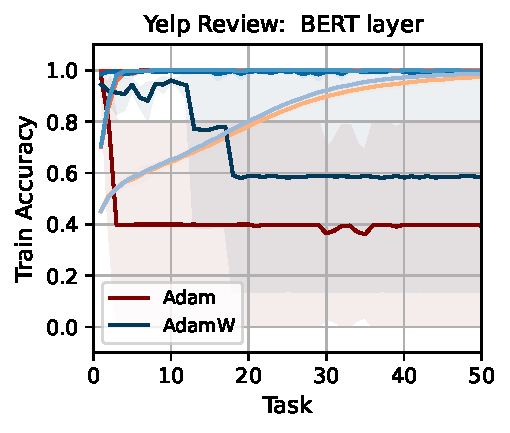
\includegraphics[width=\textwidth]{figs/Accuracy/nlp/bert_layer/yelp_review_full_40.pdf}
    }

    \caption{Accuracy of Self attenstion, Self attenstion with residual layer, and one BERT layer on NLP datasets.}
    \label{fig:nlp_self_res}
\end{figure*}




